\section{Methodology}
\subsection{Decision Trees}
\subsection{Neural Networks}
Neural networks are a type of machine learning model inspired by how the human brain works. They consist of layers of interconnected nodes, or artificial neurons, that process data, learn patterns, and make predictions. Neural networks are especially good at identifying complex relationships in data because they can model non-linear dependencies. This ability makes them ideal for tasks like image recognition, language processing, and, in our case, predicting customer churn.\\

\begin{figure}[hbt!]
    \centering
    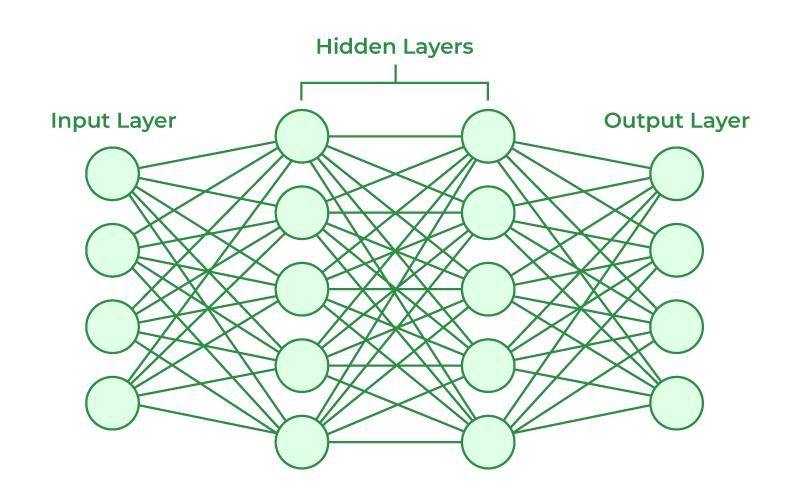
\includegraphics[width=1\linewidth]{Images/3.2.a.jpg}
    \caption{Neural Network Architecture }
    \label{fig:enter-label}
\end{figure}

The core unit of a neural network is the artificial neuron. Each neuron takes input values, computes a weighted sum, passes the result through an activation function, and produces an output. These neurons are organized into layers: the input layer takes in the raw data, hidden layers process the data by applying multiple transformations, and the output layer gives the final prediction. The network learns by adjusting its weights in a process called backpropagation, where the model tries to minimize prediction errors. This is done using optimization algorithms like stochastic gradient descent (SGD) or Adam.\\

For customer churn prediction, neural networks are particularly useful because they can capture complex patterns in customer behavior, contract details, and service usage that might not be easily identified by simpler models. The network uses activation functions like ReLU (Rectified Linear Unit) in the hidden layers to introduce non-linearity and sigmoid in the output layer to produce probabilities representing the likelihood of customer churn. The loss function typically used for training is binary cross-entropy, which measures how far the predicted values are from the actual values and helps guide the model’s learning.\\

To prevent overfitting and improve the model’s ability to generalize to new data, regularization techniques such as dropout and weight decay are often used. Additionally, hyperparameter tuning plays a critical role in optimizing the model’s performance. This includes selecting the right number of hidden layers, the number of neurons in each layer, the learning rate, and the batch size. By training on historical customer data and evaluating the model’s performance using metrics like precision, recall, F1-score, and AUC-ROC, the neural network can effectively predict the likelihood of a customer churning, which provides valuable insights for business decision-making. 
